\scanpage{112}

Regular (oriented) map\\
of the regular polygon $P_n$ $(n\geq2)$

by puncturing it at the vertices and the centers of the faces \uline{and} the midpoints of the segments

% The three small leaders belong to the three asterisks.  The small dark dot
% above the right asterisk is copied as ink, without assigning it a new meaning.
\figure{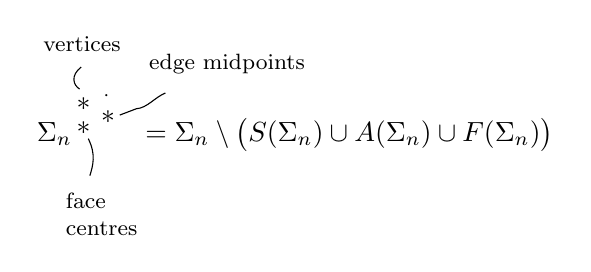
\begin{tikzpicture}[baseline=(base.base)]
\node[anchor=base] (base) at (0,0) {$\Sigma_n$};
\node at (.37,.48) {$*$};
\node at (.37,.18) {$*$};
\node at (.68,.32) {$*$};
\node at (.66,.58) {$\scriptstyle\unsure{\cdot}$};
\node[anchor=base west] at (1.03,0)
 {$=\Sigma_n\setminus\bigl(S(\Sigma_n)\cup A(\Sigma_n)\cup F(\Sigma_n)\bigr)$};
\node[font=\footnotesize,anchor=south] at (.35,1.02) {vertices};
\draw (.34,.95) .. controls (.20,.84) and (.24,.72) .. (.32,.67);
\node[font=\footnotesize,align=left,anchor=north] at (.60,-.53) {face\\centres};
\draw (.43,.04) .. controls (.53,-.16) and (.49,-.30) .. (.45,-.43);
\node[font=\footnotesize,anchor=south west] at (1.08,.74) {edge midpoints};
\draw (.83,.34) -- (1.04,.42) .. controls (1.18,.43) and (1.28,.57) .. (1.41,.62);
\end{tikzpicture}}

\unsure{divide|division} by $D_n^+\subset D_{2n}^+$

\diagram{\begin{tikzcd}[ampersand replacement=\&,column sep=large,row sep=small]
\Sigma_n^{\substack{*\\*}*}
 \arrow[r,"\deg n"] \arrow[dddd,phantom,"\rotatebox{90}{$\simeq$}" description]
 \& \Sigma_1^{\substack{*\\*}*}=\mathbb{P}_1\setminus\{\underbrace{0,\infty}_{\text{``poles''}},1,-1\}
 \arrow[r,"\deg2"]
 \& \Sigma_3^{\substack{*\\\cdot}\cdot}=U_{0\,3} \\
 \& \Vert \& \\
 \& \Sigma_n^{\substack{*\\*}*}/D_n \& \\
 \& \rotatebox{90}{$\simeq$} \& \\
\Sigma_{2n}^{\substack{*\\*}\unsure{\cdot|*}}
 \arrow[r]
 \& \Sigma_1^{\substack{*\\*}\cdot}\arrow[r,"2"]
 \& \Sigma_1^{\substack{*\\*}\cdot}\simeq U_0^3
\end{tikzcd}}

\margin{\begin{tabular}{@{}l@{}}division\\\deleted{\unsure{by the}}\end{tabular} by $D_n/D_n^+$}
\margin{(regular map $\overline{\Sigma}_{\unsure{a|\alpha}}$ with two vertices)}

division by $D_{2n}^+$

\margin{%
\figure{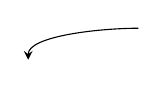
\begin{tikzpicture}[>=stealth]\draw[->] (1.4,0.4) .. controls (0.9,0.4) and (0,0.3) .. (0,0);\end{tikzpicture}}
(we have removed only the vertices and face centers)

Because of this \deleted{of} isomorphism, we let \deleted{$\unsure{D_n}$} $D_{2n}$ act on
$\Sigma_n^{\substack{*\\*}*}(\simeq\Sigma_{2n}^{\substack{*\\*}\cdot})$, we can

\unsure{therefore|of which}
}

\diagram{\begin{tikzcd}[ampersand replacement=\&,column sep=large,row sep=large]
 \& \begin{gathered}\Sigma_n^{\substack{*\\*}*}\\\simeq\Sigma_{2n}^{\substack{*\\*}\cdot}\end{gathered}
 \arrow[dl]\arrow[dr] \& \\
\Sigma_{2n}^{\substack{*\\*}\cdot}/D_{2n}^+\arrow[dd]
 \& \& \Sigma_n^{\substack{*\\*}*}/D_n^+\arrow[ll]\arrow[dl] \\
 \& \Sigma^{\substack{*\\*}*}/D_n\arrow[dl,bend left=12] \& \\
\Sigma_{2n}^{\substack{*\\*}\cdot}/D_{2n} \& \&
\end{tikzcd}}

% Curved guide from the central quotient toward the enclosed regrouping;
% it is separate from the quotient arrows.
\figure{\begin{tikzpicture}[>=stealth]\draw[->] (0,0) .. controls (0.8,0) and (1.4,0.2) .. (1.6,0.8);\end{tikzpicture}}

\diagram{\begin{tikzpicture}\node (d) at (0,0) {\begin{tikzcd}[ampersand replacement=\&,column sep=large,row sep=large]
 \& \Sigma_n^{\substack{*\\*}*}\simeq\Sigma_{2n}^{\substack{*\\*}\cdot}\arrow[d] \& \\
 \& \Sigma_n^{\substack{*\\*}*}/D_n^+\simeq\Sigma_1^{\substack{*\\*}*}\simeq\Sigma_2^{\substack{*\\*}\cdot}\arrow[dl]\arrow[dr] \& \\
\Sigma^{\substack{*\\*}\substack{*\\\unsure{*|\cdot}}}/D_{2n}^+\arrow[dr] \& \& \Sigma_n^{\substack{*\\*}*}/D_n\arrow[dl,dash] \\
 \& \Sigma_n^{\substack{*\\*}\cdot}/D_{2n} \&
\end{tikzcd}};\draw[rounded corners=22pt] (d.south west) rectangle (d.north east);\end{tikzpicture}}

\diagram{\begin{tikzcd}[ampersand replacement=\&]
\Sigma_n^{\substack{*\\*}\cdot}\arrow[r,"D_n^+"] \& \Sigma_1^{\substack{*\\*}\cdot}\simeq U_0^3
\end{tikzcd}}

If we divide by the whole of $D_n$, we find ramification under the edges

\mspage{111}
